\documentclass[german,version-2020-11]{uzl-thesis}
% !TeX program = lualatex

\UzLThesisSetup{
  Logo-Dateiname        = {institutslogo.pdf},
  Verfasst              = {am}{Institut für Informationssysteme},
  Titel auf Deutsch = { Evaluation eines Algorithmus zur Absicherung von Datenbanken mit Propabilistischen  },
  Titel auf Englisch = { Evaluation of an Algorithm for Securing Databases from Propabilsitic Inference},
  Autor                 = {Kevin Schmelzer},
  Betreuerin            = {Prof. Dr. Ralf Möller},
  Mit Unterstützung von = {Simon Schiff},
  Bachelorarbeit,
  Studiengang           = {IT-Sicherheit},
  Datum                 = {18. August 2020},
  Abstract              = {
   Englische Abstract
  },
  Zusammenfassung       = {
  	Datenbanken mit sensiblen Daten sollten einen hohen Sicherheitsstandard erfüllen. Trotzdem ist das einrichten von Sicherheitsvorkehrungen komplex und erfordert spezielle Fachkräfte, die sich mit den Systemen auskennen müssen. Diese Problematik haben viele Forschungseinrichtungen und auch Unternehmen, weil es viel zu Beachten gibt. Eins davon ist die Inferenzkontrolle für aggregierte Anfragen, wodurch ein Angreifer durch statistische Auswertungen und klug gewählte Anfragen an sensible Daten kommen kann.\\ Wir werden hierbei den Prototypen Angerona evaluieren, der Informationslücken verhindert die von probabilistischen Abhängigkeiten resultieren. Es wird gezeigt, wie man Angerona mit echten Patientendaten initalisiert und welche Vor-und Nachteile dieser Algorithmus aufweist. Zum Schluss generieren wir mit Synthea Patienten und testen die Performance mit verschiedenen Eingaben.
  },
  %Alphabetische Bibliographie
  % Alternatively:
   Numerische Bibliographie
}

\UzLStyle{alegrya modern design}


% Now, include the package you need here using \usepackage. 
\usepackage{dcolumn}
\usepackage{booktabs}
\usepackage{tikz}
\usepackage{biblatex}
\usepackage{todonotes}
\usetikzlibrary{positioning,shapes,arrows}

\newcolumntype{M}[1]{D{.}{.}{1.#1}}

\addbibresource{thesis.bib}
\begin{document}

\chapter{Einleitung}
Der Schutz von sensiblen Daten ist in vielen Bereichen wichtig, damit unbefugte nicht Daten wie Herkunft, Religion, Ethnizität usw. erhalten. Die Relevanz des Themas Privatsphäre und Digitalisierung ist spätestens seit der Wirksamkeit der Europäischen Datenschutz-Grundverordnung (DSGVO) im  Mai 2018 bemerkbar \cite{1}. Eine andere Regelung zum Schutz der Privatsphäre speziell im medizinischen Bereich ist die Health Insurance Portability and Accountability(HIPAA) aus dem Jahr 1996. Hierbei wurde für jeden der im Gesundheitswesen tätig ist in den USA durch bestimmte Anordnungen und Regelungen vorgeschrieben, die Privatsphäre der Patienten durch z.B. Zugangskontrolle, Anonymisierung, richtige Datenspeicherung usw. zu schützen. \cite{7}[ Dabei kam es damals schon zum Konflikt zwischen dem Schutz der Privatsphäre und zur Verwendung oder Veröffentlichung von Gesundheitsinformation um wichtige soziale Ziele, wie zum Beispiel Forschungszwecke, zu erfüllen.\cite{8}. Der bisherige Ansatz sensible Daten zu schützen war es den Zugang in teilen einfach zu verbieten und die Daten zu anonymisieren \cite{2}. Dieser Ansatz ist zwar für die Sicherheit optimal, jedoch leidet darunter das andere Konfliktziel.] \\ 
Um die Vertraulichkeit von sensiblen Daten zu wahren braucht man hingegen Schutz vor direkten und indirekten Zugriff auf die Datenbank. Beim Direkten Zugang versucht ein Nutzer aus Datenbankantworten und indirekter Zugang ein Nutzer durch statistische Auswertungen von externen Informationen und klug gewählte Anfragen an sensible Daten zu kommen.  Daher kam es zu einigen neuen Ansätzen, die auch den indirekten Zugang schützen sollen und eine davon ist die Database Inference Control (DBIC). Damit DBIC auch effektiv den indirekten Zugang verhindert, muss dieser eine große Menge von probabilistischen Abhängigkeiten abdecken können, um viele verschiedene Angreifermodelle darzustellen und es muss eine angemessene Laufzeit aufweisen, um diese auch auf Reale und große Datenbanken anwenden zu können.\\
Dies wurde mit Angerona versucht, da bisherige DBIC Mechanismen nur präzise Datenabhängigkeiten oder nur eine begrenzte Anzahl von probabilistischen Abhängigkeiten erlaubt haben und somit nicht für Reale Datenbanken tauglich waren. \cite{6}
\\ \\

\todo[inline, size=\tiny]{relevante daten und anonymisierung, Warum angreifer modeliert? (Vorwissen) 
	warum ich gerade medizinische DB verwendet habe?}

\section{Beiträge dieser Arbeit}
TODO
In dieser Arbeit wird der Prototyp von Angerona, einem [Beschreibung für Angerona] von Marco Guarnieri evaluiert auf echten, anonymisierten Patientendatenbanken. Dabei werden wir im ersten Schritt  die Initialisierung von Angerona vorstellen und anschließend mit realistischen Beispielen bewerten. Zum Schluss wird die Laufzeit bei verschiedenen Eingaben gezeigt.


\section{Verwandte Arbeiten}
Informationsverlust verhindern durch Probabilistische Abhängigkeiten in Datenbanken zu verhindern haben schon einige versucht. Einige Ansätze davon sind : [ ANSÄTZE SUCHEN]. Die am nächsten verwandte Arbeit ist selbstverständlich die von Marco Guarnieri, Srdjan Marinovic und David Basin, weil ich hierbei das von Ihnen entworfene Framework/Programm evaluiere. Für Angerona habe ich mich entschieden, weil der der beste ist[Guten grund finden usw. und mit anderne vergleichen, andere related works aber warum genau marcos?]


\section{Aufbau dieser Arbeit}
% Replace the following by one or two paragraphs describing the
% thesis's structure.
In dieser Arbeit werden wir zuerst Angerona vorstellen und einige Beispiele zeigen die den Zweck des Algortithmus näher bringen. Anschließend folgen die Ergebnisse und Auswertungen dieser Arbeit gefolgt von den Benchmarks.
\chapter{Vorbereitung von Angerona}
\section{Grundlegendes}
\subsection{Datenbanksystem}
\begin{figure}[ht]
	\centering
	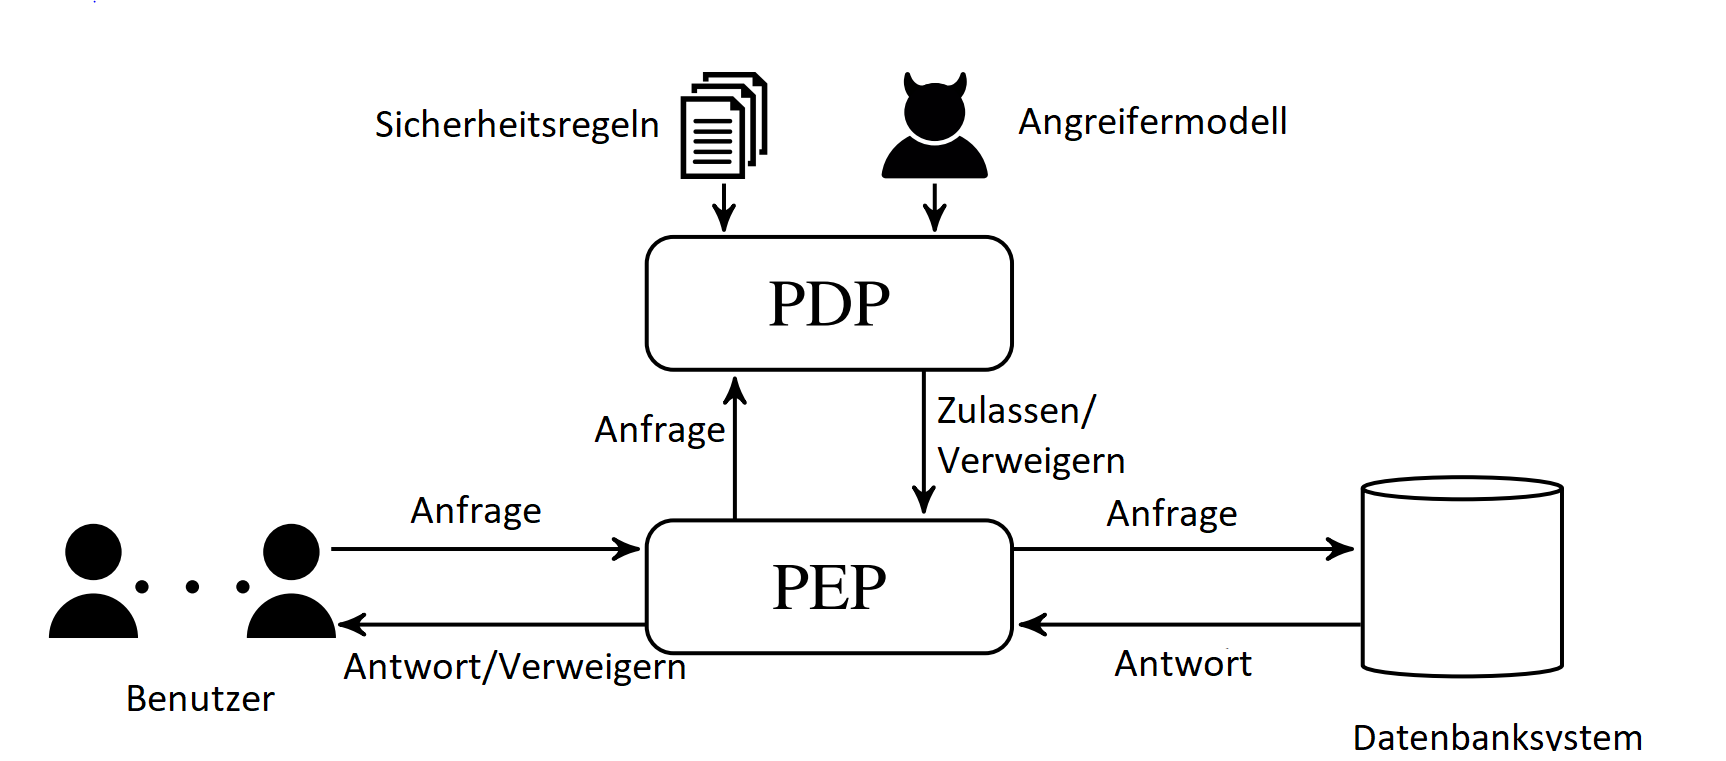
\includegraphics[width=0.6\textwidth]{System-model.PNG}
	\caption{Systemmodell}
	\label{fig1}
	\end{figure}
Die Abbildung 2.1 zeigt das von Angerona genutzte Systemmodell. Dabei interagiert der Nutzer mit zwei Komponenten und zwar dem Datenbanksystem und dem Inferenzkontrollsystem, welches aus dem Policy Decision Point(PDP) und dem Policy Enforcement Point (PEP) besteht. Diese entscheiden Anhand von den Sicherheitsregeln und dem Angreifermodell, ob die Anfrage an das Datenbanksystem übergeben wird und der Nutzer eine Antwort erhält oder ob die Anfrage verweigert wird. Dabei gehen wir davon aus, dass alle Kommunikationskanäle über sichere Kanäle laufen. \\ \\ 
\textbf{Datenbanksytem} Das Datenbanksystem handhabt die Systemdaten und ordnet die Tabellen auf Tupel um.    \\  
\textbf{Benutzer} Jeder Nutzer hat ein eigenes Konto um Informationen mithilfe von \textit{SELECT} Anfragen an das Datenbanksystem zu stellen. Dabei hat jeder nutzer nur Leserechte und kann die Datenbank nicht verändern. Jede Anfrage wird vom Inferenzkontrollsystem geprüft und wird nur ausgeführt, wenn diese von den Sicherheitsregeln autorisiert wird. \\ 
\textbf{Sicherheitsregeln} Besteht aus einer Menge von negativen Genehmigungen, die Informationen geheim halten sollen. Diese Genehmigungen definieren die Erwartungen[Vlt. anderes Wort?] jedes Benutzers über den Inhalt der Datenbank als Wahrscheinlichkeitsverteilung. Die negativen Genehmigungen werden formalisiert durch ein Kommando in der Form \textit{SECRET q FOR u THRESHOLD l}, wobei q die Anfrage, u den Benutzer und l die Grenze darstellt, bei der die Anfrage genehmigt werden darf. Dabei gilft 0 \leq l \leq 1. Eine Sicherheitsregel "Der Benutzer u ist nicht autorisiert die Antwort von der Anfrage q zu erfahren" kann ausgedrückt werden mit \textit{SECRET q FOR u THRESHOLD 1}. Außerdem kann die Regel "Für alle Benutzer $u \notin \{u1,...,u_n\}$, muss die Erwartung von u bei der Anfrage q kleiner als l sein" mit dem Kommando \textit{SECRET q FOR USERS NOT IN $\{u_1,...,u_n\}$ THRESHOLD l}\\ 
\textbf{Angreifer} Ein potentieller Angreifer ist jeder Benutzer im Datenbanksystem mit einem Benutzerkonto. Das Ziel eines Angreifers ist es die Sicherheitsregeln zu verletzen indem er mindestens auf ein \textit{SECRET} schließen kann mit einer Wahrscheinlichkeit über dem dazugehörigen \textit{THRESHOLD}. \\ Der Angreifer interagiert mit dem System, indem er Anfragen stellt und kann mithilfe der Antworten das Verhalten beobachten. Außerdem kann er die dadurch erlangten Informationen nutzen um Beziehungen zwischen den Daten festzustellen. Wir gehen davon aus, dass der Angreifer das Datenbankschema und die  Integritätsbedingungen kennt. \\
\textbf{Datenbankzustand} Der Datenbankzustand repräsentiert die Belegung der Datenelemente in der Datenbank. \\
\textbf{Angreifermodell} Das Angreifermodell repräsentiert die initiale Erwartung des Benutzers über den aktuellen Datenbankzustand und wie dieses sich verändert, wenn der Benutzer mit der Datenbank interagiert. Diese Erwartung kann das Wissen des Angreifers über die Beziehung zwischen den Datenelementen oder Vorwissen widerspiegeln.\\ 
\textbf{Inferenzkontrollsystem} Das Inferenzkontrollsystem schützt die Vertraulichkeit der Daten in der Datenbank. Es besteht aus dem PEP und dem PDP und wird mit den Sicherheitsregeln P und dem Angreifermodell \textit{ATK} konfiguriert. Für jeden Benutzer behält das Inferenzkontrollsystem die Erwartung gemäß ATK im Überblick.  \\
Das System fängt alle Anfragen $c$ vom Benutzer $u$ ab und entscheidet dann ob $u$ autorisiert ist $c$ auszuführen. Wenn $c$ die Sicherheitsregeln erfüllt, dann wird $c$ an das Datenbanksystem weitergeleitet, dass dann $c$ ausführt und die Antwort an $u$ zurückgibt. Andernfalls wird eine \textit{security exception} ausgelöst und $c$ wird verweigert. \cite{6}
\subsection{Bayes-Netze}
Bevor wir anfangen können das Projekt zu initialisieren, sollten wir uns mit Bayes-Netzen vertraut machen. Für jede Implementierung, die wir in Angerona vornehmen wollen, sollten wir ein dazugehöriges Bayes-Netz modellieren, damit wir die Abhängigkeiten übersichtlich sehen und es wird uns leichter fallen die InitStatements und das beliefProgram(Kapitel 2.2.1) zu deklarieren bzw. es wird fast unmöglich ohne Bayes-Netz bei komplexeren Abhängigkeiten überhaupt diese zu deklarieren. \\ 
Ein Bayes-Netz ist ein direkter, azyklischer Graph in dem jeder Knoten die gemeinsamen Wahrscheinlichkeitsverteilung jeder Zufallsvariablen enthält. Dabei ist jeder Knoten selbst eine Zufallsvariable mit einer Wahrscheinlichkeitsverteilung $P(V_i \mid Parent(V_i) )$. Die Elternbeziehung eines Knoten gibt dabei an, dass $Parent(V_i) $ einen direkten Einfluss auf $V_i$ hat und wird  mit einem gerichteten Pfeil dargestellt\cite{3} Eine Modellierung für ein Bayes-Netz sieht man in Abbildung 2. \\ 

\subsection{Problog}
Problog ist eine probabilistische Erweiterung von Prolog(PROgramming in LOGic), wobei Prolog eine logische Programmiersprache ist, die aus verschiedenen Klauseln $k_i$ und aus logischen Verknüpfungen ein Ergebnis berechnet. Problog erweitert jedes $k_i$ mit einer Wahrscheinlichkeit $p_i$, wodurch Problog uns Wahrscheinlichkeiten ausgibt, mit welcher die $k_i$ eintreten,wohingegen  Prolog uns nur ein true oder false nach logischen Berechnungen liefern könnte. \\ 
\textbf{Beispiel 1}: einfaches Problog Programm
\uzldeflanguageshorthand{Problog}{style=code,language=problog}
\begin{Pseudocode}
1	0.1::erdbeben.
2	0.9::alarm_bei_erdbeben.
3	alarm :- erdbeben, alarm_bei_erdbeben.
\end{Pseudocode} 
Ein Problog Programm $T = {p_1 :: k_1, ... p_n :: k_n}$ gibt somit eine probabilistische Verteilung über die einzelnen Klauseln und diese können anschließend zu einer beliebigen Logischen Verknüpfungen aus $K = {k_1 , ... , k_n}$ verknüpft werden. In Beispiel 1 sehen wir, dass der Fakt \textit{erdbeben} mit Wahrscheinlichkeit $0.1$ wahr ist und $0.9$ falsch ist. Andersrum für den Fakt alarm\_bei\_erdbeben haben wir eine Wahrscheinlichkeit $0.9$, dass der Alarm auslöst und eine Gegenwahrscheinlichkeit von $0.1$, dass dieser nicht auslöst. Diese Aussagen aus Zeile 1 und 2 nennt man auch probabilistischer Fakt.\\  In Beispiel 1 haben wir somit für die Klausel $k_{alarm} = 0.9 \cdot 0.1 = 0.09  $. \cite{4}\cite{5} \\ 
In unserem Fall benötigen wir als logische Verknüpfung nur das $\land$, dass in Problog mit einem $","$ dargestellt wird. Normalerweise wird eine Negation mit $"\textbackslash+"$ gekennzeichnet, in Angerona jedoch mit $"NOT"$.\\ \\
Noch ein sinnvolles Konstrukt, dass von Problog geliefert wird ist die annotated disjunction, die es möglich macht auch nicht binäre Entscheidung abzubilden. Ein Beispiel dafür wäre ein Alarm, der die Werte $A_1$ = an zu 0.2  $A_2$ = aus zu 0.7 oder $A_3$ = defekt zu 0.1 annehmen kann. Dies würde man mithilfe der annotated disjunction folgendermaßen formulieren : 
\begin{Pseudocode}
2/10::alarm(X, 1); 7/10::alarm(X, 2); 1/10::alarm(X, 3).
\end{Pseudocode}

\subsection{Polytree}
Ein Polytree ist ein direkter, azyklischer Graph, der azyklisch bleibt, selbst wenn wir alle direkten Kanten durch indirekte Kanten ersetzen.
\subsection{Angerona}
Angerona ist ein DBIC(Database Inference Control) Mechanismus der Datenbanken gegen probabilistische Inferenzen absichert. Hierbei betrachten wir nur einen Prototypen von Angerona, da es noch keine vollendete Version gibt. Der Prototyp unterstützt heribei nur boolische Anfragen. Es wurde zwar eine Lösung für nicht-boolische Werte im Paper vorgestellt, jedoch wurde diese nicht im Prototypen implementiert.\\ 
 Als input benötigt Angerona ein Angreifermodell, dass die Erwartung des Angreifers repräsentiert und nutzt dafür Problog.  Angerona prüft dabei für jede Anfrage q, ob diese ein vorher definiertes Geheimnis $g \in G$ verletzt. Dabei wird zuerst geprüft, ob g bereits vorher verletzt wurde. Wenn dies nicht der Fall ist, dann wird geprüft, ob nach der Antwort von q ein anderes Secret $g' \in G$  verletzt wird. Dafür wird jedoch geprüft, ob die Erwartung von dem Benutzer u über $g'$ und $g$  unter dem definierten Threshhold liegt, wenn die Anfrage q ausgeführt und wenn q nicht ausgeführt wird. Damit verhindert Angerona, dass seine Entscheidung nicht weitere Secrets verletzt und somit sensible Informationen veröffentlicht.  \\ Geprüft wird dies, indem Angerona zuerst prüft, ob es überhaupt möglich ist, dass die Anfrage q in einem beliebigen Datenbankzustand zutreffen könnte. Wenn dies der Fall ist, dann wird die Historie h, die alle getätigten Anfragen zu jedem Nutzer speichert , erweitert mit der Anfrage q und prüft dann anschließend ob mit der erweiterten Historie einen Datenbankzustand gibt, indem q nicht zugelassen wird. \cite{6}


\section{Praktisches Setup}
Um die folgenden Experimente und Auswertung zu reproduzieren, sollten wir erst mal die Anwendungen und Einstellungen vorstellen. Der genutzte Computer hat einen AMD Ryzen 2600x Sechs-Kern Prozessor die mit 3.6GHz laufen, 16GB RAM mit 2400MHz und nutzt Windows
10 Enterprise LTSC als Betriebssystem. Das Projekt wurde jedoch aus Kompatibilitätsgründen auf einer virtuellen Maschine ausgeführt. Die VM läuft auf Oracle VM VirtualBox Version 6.1.6 und nutzt Ubuntu 20.04.1 LTS. Dabei wurden der VM Sechs von Zwölf Threads und 8GB RAM bereitgestellt. \\ \\
Nun fangen wir an den Prototypen von Angerona zu initialisieren.
Der Prototyp lässt sich auf der Seite von Marco Guarnieri \cite{6} herunterladen. Angerona lässt sich in zwei verschiedene Modis starten :
\begin{enumerate}
	\item Experiment: Hiermit können vorgefertigte Beispiele aus dem Paper \"Securing Databases from Probabilistic Inference" \cite{6} reproduziert werde. Hierbei werden keine größeren Initialiserungsschritte benötigt und es wird für einen das das beliefProgram und die dazugehörige Datenbank generiert. Anschließend werden zufällig generierte Anfragen an die Datenbank gestellt und von Angerona geprüft. Als output erhält man die Zeitmessung für die ausführung der Anfrage, die Ausführungszeit von Angerona und die gesamte Inferenzzeit[TODO genauer]	in einer CSV Datei.
	\item Manual: Erlaubt es mit einer Datenbank zu interagieren, die durch Angerona geschützt ist. Dieser Modus erfordert drei Dateien als input und zwar das BeliefProgram, initStatements und das template. Diese drei Dateien werden wir im folgenden weiter erläutern.
\end{enumerate}
Wir verwenden in unserem Fall ausschließlich den Manual mode.
\subsection{BeliefProgram}
Das beliefProgram.pbl beschreibt das Angreifermodell. Hier werden die Erwartungen des Angreifers mithilfe von Problog beschrieben. \\ 
In die ersten Zeilen schreiben wir dabei alle unsere Knoten $\{v_0,...,v_n\} \in V$ aus dem Bayes-Netz hin, die keine Abhängigkeit haben, in der Form
% darf man das so schreiben? Hab versucht das gut auszudrücken oder lieber natürliche Sprache ?
\begin{Pseudocode}
$np_0.name(X) :- p\_np_0.name(X).$ 
...
$np_n.name(X) :- p\_np_n.name(X).$ 
\end{Pseudocode}
, wobei $\{np_i \in V \mid Parent(np_i) = \emptyset\}$ und das Attribut name gibt einfach den vorher definierten Namen für den Knoten aus. Anschließend schreiben wir die Wahrscheinlichkeit für die Klausel $p\_np_0.name$ als probabilistischen Fakt hinzu in der Form :
\begin{Pseudocode}
$P(np_0) ::  p\_np_0.name(X).$ 
...
$P(np_n) ::  p\_np_n.name(X).$ 
\end{Pseudocode} $ $\\
Für die Knoten mit Abhängigkeiten, also für alle Knoten V für die gilt $H=\{v \in V | \vert Parent(v) \vert \geq 1 \}$ schreiben wir die Klausel für jede möglich Welt von den Abhängigkeiten hin und verknüpfen diese mit einer Konjunktion, die in Problog mit einem $","$ dargestellt wird. Die Negation stellen wir nicht wie üblich in Problog mit einem $\backslash +$, sondern mit einem NOT da. Anschließend konjugieren wir jeden Ausdruck mit einer selbst definierten Variable, der wir am Ende durch einen probabilistischen Fakt die dazugehörige Wahrscheinlichkeit für diese Welt geben. \\ \\
Wenn eine variable anstatt zwei Wahrheitswerte true und false auch mehr Werte zulässt. nennen wir diese mehrwertige Variable.
Um diese im BeliefProgram auszudrücken, wird der mehrwertigen Variable in eine annotated disjunction eingeteilt. Jedoch wird dann das $;$ entfernt und für jeden Wert den die Variable annehmen kann eine neue Klausel erstellt mit einer neuen Variable die wir im folgenden $sw_1, ... sw_n$ nennen und fügen zum Schluss für jeder dieser neu erstellen Variable ein Probabilistischen Fakt hinzu mit der dazugehörigen Wahrscheinlichkeit mit der der Wert zutrifft.
Den Namen der mehrwertigen Variable definieren im folgenden als $A$ und die tupel, die durch die annotated disjunctiuon übergeben werden als $t_1 ,..., t_n$. Somit würden wir dann folgendes erhalten, wenn wir die annotated disjunction für das beliefProgram angepasst ausführen:
\begin{Pseudocode}
$A(t_1)$ :- $sw_1(t_1)$
...
$A(t_n)$ :- NOT $sw_1(t_1), ... ,$ NOT $sw_{n−1}(t_{n−1}), sw_n(t_n)$

$p_1::sw_1( )$
...
$p_n::sw_n( )$

\end{Pseudocode}
\subsection{InitStatements}
Die InitStatements.txt definieren das Datenbankschema und füllen die Datenbank mit den benötigten Werten. Außerdem werden hier die Regeln definiert, zu welchen Bedingungen ein Nutzer/Angreifer auf die Datenbank zugreifen darf. \\ 
Die InitStatements können in vier Schritten initalisiert werden:
\begin{enumerate}
	\item \textbf{Tabellen }initialisieren mit dem Kommando \textit{AS admin : CREATE TABLE tablename(parameter)}.
	\item  \textbf{Benutzer  }initialisieren mit dem kommando \textit{AS admin : ADD USER benutzer}
	\item \textbf{Sicherheitsregeln} definieren mit \textit{AS admin : SECRET anfrage('id') FOR benutzer THRESHOLD grenze}
	\item \textbf{Füllen} der Datenbank mit \textit{AS admin : INSERT IN tabelle ['id']}
\end{enumerate} 

\subsection{Template}
Die template.cpt ist die Vorlage für Angerona. In dieser werden die Tabellen aus den InitStatements und die definierten Fakten aus dem BeliefProgram einfach mit einem leeren Array initalisiert.
\section{Beispiel}
Wir betrachten eine Datenbank, die das Rauchverhalten und die Elternbeziehung von Patienten speichert und ob diese Lungenkrebs haben. Die Datenbank hat dabei die Tabellen \textit{Patienten, Raucher, Lungenkrebs, } und \textit{Elternteil-hat-Krebs}. Außerdem betrachten wir folgendes Probabilistisches Modell: 
\begin{enumerate}
\item Jeder Patient entwickelt mit einer Wahrscheinlichkeit von 5\% Krebs
\item Wenn ein Elternteil Lungenkrebs hat, dann steigt die Wahrscheinlichkeit vom Kind Lungenkrebs zu bekommen um 20\%
\item Wenn ein Patient raucht, dann steigt die Wahrscheinlichkeit für Lungenkrebs um 25\%
\end{enumerate}
Zu Beginn übertragen wir das Probabilistische Modell in ein Bayes-Netz.  \\
\begin{tikzpicture}[
	node distance=1cm and 0cm,
	mynode/.style={draw,ellipse,text width=2cm,align=center}
	]
	\node[mynode] (patient) {Patienten};
	\node[mynode,right=of patient] (smokes) {Raucher};
	\node[mynode,right=of smokes] (parent) {Elternteil-hat-krebs};
	\node[mynode,below right=of patient] (cancer) {Lungenkrebs};
	\path 
	(patient) edge[-latex] (cancer)
	(smokes) edge[-latex] (cancer) 
	(parent) edge[latex-] (cancer);
	\node[above=0.5cm of patient]
	{
		\begin{tabular}{cM{1}M{1}}
			\toprule
			\multicolumn{1}{c}{Patienten} \\
			\multicolumn{1}{c}{$P(P)$} \\
			\cmidrule(r){1-1}
			$1.00$\\
			\bottomrule
		\end{tabular}
	};
	\node[above=0.5cm of smokes]
	{
		\begin{tabular}{M{1}M{1}}
			\toprule
			\multicolumn{1}{c}{Raucher} \\
			\multicolumn{1}{c}{$P(R)$} \\
			\cmidrule(r){1-1}
			$0.23$ \\
			\bottomrule
		\end{tabular}
	};
	\node[above=0.5cm of parent]
	{
		\begin{tabular}{ccM{1}M{1}}
			\toprule
			\multicolumn{1}{c}{Elternteil hat Krebs} \\
			\multicolumn{1}{c}{$P(E)$} \\
			\cmidrule(r){1-1}
			$0.1$ \\
			\bottomrule
		\end{tabular}
	};
	\node[below=0.5cm of cancer]
{
	\begin{tabular}{ccM{4}M{4}}
		\toprule
		\multicolumn{1}{c}{Lungenkrebs} \\
		\multicolumn{1}{c}{P} &	\multicolumn{1}{c}{E} & \multicolumn{1}{c}{R} & \multicolumn{1}{c}{$P(L)$} \\
		\cmidrule(r){1-4} 
		T&T&T& $0.5$ \\
		T&T&F& $0.25$ \\
		T&F&T& $0.3$ \\
		T&F&F& $0.05$ \\
		F&T&T& $0.1$ \\
		F&T&F& $0.1$ \\
		F&F&T& $0.1$ \\
		F&F&F& $0.1$ \\

		\bottomrule
	\end{tabular}
};
	
\end{tikzpicture}


\chapter{Ergebnisse und Auswertung}
\section{mimic}
\section{eicu}
\section{synthea}
% Lifecycle.java die uuid zu Biginteger umwandeln und blabla. guck nochmal
\section{Angreifer modellierung}
\section{Vor und nachteile}

\chapter{Benchmarks mit Patientendatenbanken}



\chapter{Zusammenfassung und Ausblick}

% !!!!!!!!!!!!!!!!!!!!!!!!!!!!!!!!!!
% !!! Your action is needed here !!!
% !!!!!!!!!!!!!!!!!!!!!!!!!!!!!!!!!!
%
% Replace the following with your conclusion
% Ausblick : Gruppensystem einführen vlt. Vlt ist es jetzt schon möglich?, damit nicht jeder einzelnd deklariert werden muss weil sonst sau voll , 2. Nachteil : nur Numbers/integers erlaubt und z.B. standard uuid ist ein mix aus Buchstaben , Nummern und -(Sonderzeichen)


This template document got much longer than I had initially intended
with more and more hints and comments becoming part of the text. The
reason is, of course, that writing a thesis is not easy since there
are a \emph{lot} of things to consider. However, you have six months
to write your thesis, so you stand a decent chance to get most things 
right.

Do some great scientific research now and report on it in a thesis
that is a pleasure to read. 


\listoftodos



% Normally, the bibliography comes next at this point. Do *not* (try
% to) include further indices and tables like an index or
% a list of figures or a list of tables or such things. Nobody
% actually uses them and they just use up space. 
%
% You *can* however include a glossary, if this seems appropriate. It
% goes here as an unnumbered chapter. Most thesis will *not* need a
% glossary: a well-written text (re)explains strange words and
% concepts as necessary. However, there are situations where a
% glossary may be helpful.














%%%
% 
% Bibliographies
%
%%%
%
% The uzl-thesis class will load biblatex for the bibliography
% management. This is a powerful package, see its documentation for
% details. The styles will be setup correctly and automatically by
% choosing one of the two style keys as described earlier.
%
% In order for the bibliography to work, run latex in the following
% order (which is the standard order):
% 
% > lualatex thesis-example
% > bibtex thesis-example
% > lualatex thesis-example
% 
% Add BibTeX files using \addbibresource or use the {bibtex entries}
% environment (see below).
%
%%%
%
% Although everyting is normally setup automatically, you can change
% the options passed to biblatex using the key 'biblatex';
% for instance,
%
%   \UzLThesisSetup{biblatex={firstinits=false}}
%
% will switch off shortened first names. Normally, you will not need
% this key in your preamble. 
% 
% Note that the bibtex program is used as the 'backend' of biblatex
% by default (rather than biber, which is the preferred program of
% biblatex). This means that you can (and must) run *bibtex* after you
% have run lualatex on your thesis. If you wish to use biber instead
% of bibtex, say 'biblatex={backend=biber}'. 
% 
%%%
%
% The following environment is optional. It allows you to keep the
% bibtex entries for your thesis right here in the thesis file. What
% happens is that each time this tex file is processed, the contents
% of the following environment gets written to the file
% \jobname-bibtex-entries.bib (this file gets overwritten each
% time). Independently, \addbibresource{\jobname-bibtex-entries.bib}
% is always called if the file \jobname-bibtex-entries.bib
% exists. 
%
% In result, you can edit and keep the bibliography's bibtex entries
% right here. If you change something here, run latex, then bibtex,
% then latex once more.
%
% If you would like to manage the bibtex entries in a separate file,
% remove the below environment, delete the \jobname-bibtex-entries.bib
% file and instead write
%
% \addbibresource{filename-of-your-bibtex-file.bib}
%
% in the preamble.
%
%%%


% !!!!!!!!!!!!!!!!!!!!!!!!!!!!!!!!!!
% !!! Your action is needed here !!!
% !!!!!!!!!!!!!!!!!!!!!!!!!!!!!!!!!!
%
% Replace following example entries with the ones of your thesis.



% If you need to have an appendix (I advise against it), insert it
% here using, first, \appendix and then \chapter and then,
% possibly, \section. 
%
% \appendix
%
% \chapter{Technical Appendix}
%
% \section{Experimental Parameters} % possibly
%
% Again, I advise against using an appendix.


\end{document}

%  LocalWords:  LaTeX tex moretexcs Lübeck pdf uzl lualatex bibtex th
%  LocalWords:  TechReport Kernighan Lamport's Tantau's Tantau cls kZ
%  LocalWords:  Mustermann emacs oldschool pdflatex texmf utf biber
%  LocalWords:  biblatex Alphabetische Bibliographie Numerische VIIa
%  LocalWords:  varioref german Einleitung Beiträge dieser Arbeit xml
%  LocalWords:  Ergebnisse Verwandte Arbeiten Aufbau nucleotide VIIc
%  LocalWords:  ensembl amino phylogenetic Alexa Siri decrypt versa
%  LocalWords:  cryptographic pre nondeterministic deterministically
%  LocalWords:  Beutelspacher Untersuchungen zum genetischen sep llcc
%  LocalWords:  Beispiel tikz jpg png Alegrya Kasimir Malewitsch PGF
%  LocalWords:  Lamport Institut für Theoretische Informatik zu url
%  LocalWords:  Universität Springer DowneyF Downey Parameterized doi
%  LocalWords:  BibLaTeX Kime Philipp urldate Mittelbach hyperref Lua
%  LocalWords:  Rahtz Oberdiek Heiko Braams Bezos López fontspec Das
%  LocalWords:  Arseneau amsmath ist Tipps und zur Formulierung
%  LocalWords:  mathematischer Gedanken Mathematik Studienanfänger
%  LocalWords:  Albrecht Vieweg Teubner Verlag
